%%%%%%%%%%%%%%%%%%%%%
%   AMS packages    %
%%%%%%%%%%%%%%%%%%%%%
\documentclass{beamer}
\usepackage{amsmath}
\usepackage{amsxtra}
\usepackage{amscd}
\usepackage{amsthm}
\usepackage{amsfonts}
\usepackage{amssymb}
\usepackage{eucal}
%\usepackage[all]{xy}
\usepackage{graphicx}
\usepackage{comment}
\usepackage{amssymb}
\usepackage{mathrsfs}
\usepackage{latexsym,amsmath,amscd,amssymb,epsfig,verbatim}
\usepackage{tikz}
\usetikzlibrary{arrows,shapes}
\usepackage{tikz-qtree}
\tikzset{level distance=50pt,
    sibling distance=7pt,
    every tree node/.style={align=center},}

\newtheorem{thm}{Theorem}
\newtheorem{cor}[thm]{Corollary}
\newtheorem{lem}[thm]{Lemma}
\newtheorem{prop}[thm]{Proposition}
\newtheorem{ex}[thm]{Exercise}
\newtheorem{conjecture}{Conjecture}
%\newtheorem*{conjecture*}{Conjecture}

\theoremstyle{remark}
\newtheorem{rem}[thm]{Remark}
\newtheorem{eg}[thm]{Example}
%\newtheorem{fact}[thm]{Fact}

%\newtheorem{counterexample}[thm]{Counterexample}
\newtheorem{defn}[thm]{Definition}
%\newtheorem{claim}[thm]{Claim}
%\newtheorem{note}[thm]{Notation}
%\newtheorem{warning}[thm]{Warning}
%\newtheorem{variant}[thm]{Variant}
%\newtheorem{question}[thm]{Question}
%\newtheorem{construction}[thm]{Construction}
%\newtheorem{terminology}[thm]{Terminology}
%\newtheorem{convention}[thm]{Convention}

%%%%%%%%%%%%%%%%%%%%%%%%% custom commands %%%%%%%%%%%%%%%%%%%%%%%%%%%

\newcommand\nc{\newcommand}
\nc\on{\operatorname}
\nc\renc{\renewcommand}
\newcommand\ssec{\subsection}
\newcommand\sssec{\subsubsection}
\newcommand\BH{{\mathbb H}}
\newcommand\bO{{\mathbf O}}
\newcommand\CC{{\mathcal C}}
\newcommand\CH{{\mathcal H}}
\newcommand\BN{{\mathbb N}}
\newcommand\BC{{\mathbb C}}
\newcommand\BF{{\mathbb F}}
\newcommand\BR{{\mathbb R}}
\newcommand\BQ{{\mathbb Q}}
\newcommand\BP{{\mathbb P}}
\newcommand\BBZ{{\mathbb Z}}
\newcommand\uR{\underline{R}}
\newcommand\uZ{\underline{\BBZ}}
\newcommand\CF{{\mathcal F}}
\newcommand\uCF{\underline{{\mathcal F}}}
\newcommand\BZ{{\mathbb Z}}
\newcommand\BA{{\mathbb A}}
\newcommand\fa{{\mathfrak a}}
\newcommand\fp{{\mathfrak p}}
\newcommand\fq{{\mathfrak q}}
\newcommand\fm{{\mathfrak m}}
\newcommand\so{{\mathscr O}}
\newcommand\sg{{\mathscr G}}
\newcommand \sx{{\mathscr X}}
\newcommand \sy{{\mathscr Y}}

\newcommand\scm{{\mathscr M}}
\newcommand\scn{{\mathscr N}}
\newcommand\scf{{\mathscr F}}
\newcommand\scg{{\mathscr G}}
\newcommand\sco{{\mathscr O}}
\newcommand\sch{{\mathscr H}}
\newcommand\scl{{\mathscr L}}
\newcommand\sci{{\mathscr I}}

\newcommand{\id}{\mathrm{id}}
\newcommand\im{\text{im }}
\newcommand\coker{\text{coker}}
\newcommand \spec{\text{Spec }}
\newcommand \proj{\text{Proj }}
\newcommand \rspec{\textit{Spec }}
\newcommand \rproj{\textit{Proj }}
\newcommand{\gal}{\mathrm{Gal}}

\newcommand \trdeg{\text{tr. deg }}
\newcommand \codim{\text{codim}}
\newcommand \rk{\text{rk }}
\DeclareMathOperator\di{Div}
\newcommand \depth{\text{depth }}
\DeclareMathOperator{\ord}{ord}
\DeclareMathOperator{\sym}{Sym}


%%%%%%%%%%%%%%%%%%%%% cring custom commands %%%%%%%%%%%%%%%%%%%%%%%%%

\newcommand \subhalf[1]{\frac{{#1} - 1}{2{#1}}}
\newcommand{\se}[1]{\section*{Problem #1}}
\newcommand{\halfcan}{L}
\DeclareMathOperator{\Supp}{Supp}
\DeclareMathOperator{\initial}{in_\prec}
\DeclareMathOperator{\gin}{gin}
\DeclareMathOperator{\Eff}{Eff}
\DeclareMathOperator{\sat}{sat}

\newcommand{\GL}{\operatorname{GL}}
\newcommand{\SL}{\operatorname{SL}}
\newcommand{\PGL}{\operatorname{PGL}}
\newcommand{\PSL}{\operatorname{PSL}}

\newcommand\Bk{{\Bbbk}}


\newcommand\Wider[2][3em]{%
\makebox[\linewidth][c]{%
  \begin{minipage}{\dimexpr\textwidth+#1\relax}
  \raggedright#2
  \end{minipage}%
  }%
}


\AtBeginSection[]{
	\begin{frame}{Outline of Talk}
		\tableofcontents[currentsection]
	\end{frame}
}

\beamertemplatenavigationsymbolsempty

%\usepackage{beamerthemeshadow}

\mode<presentation>{}
\usetheme{CambridgeUS}
\usecolortheme{beaver}

%%%%%%%%%%%%   Title slide info  %%%%%%%%%%%%%
\title{Spin Canonical Rings of Log Stacky Curves}

%\author[A. Landesman, P. Ruhm, and R. Zhang]{Aaron Landesman\inst{1}, Peter Ruhm\inst{2}, Robin Zhang\inst{3}}
 %
%\institute[] % (optional)
%{
  %\inst{1}
	%Harvard University
	%,
  %\inst{2}
	%Stanford University
  %,
  %\inst{3}
	%Stanford University
%}

\author[A. Landesman, P. Ruhm, and R. Zhang]{
Aaron Landesman (Harvard University) \\
Peter Ruhm (Stanford University) \\
Robin Zhang (Stanford University)
}

\date[July 17, 2015]{
Emory University Number Theory REU, Atlanta, GA\\
\mbox{}\\
July 17, 2015\\
\mbox{}\\
% \tiny{Slides available at \url{http://www.mathcs.emory.edu/~dzb/slides/} }
}

\begin{document}

%%%%%%%%%%%%  Title Frame  %%%%%%%%%%%%%%%%
\begin{frame}
	\titlepage
\end{frame}

%%%%%%%%%%%%%%%%%%%%   Modular Forms Section   %%%%%%%%%%%%%%%%%%%
\section{Modular Forms} 

\begin{frame}{Fuchsian Group}
%Consider rings of modular forms of Fuchsian groups.
%\pause

\begin{defn}
{\bf Fuchsian Group}: a discrete subgroup $\Gamma \subseteq \PSL_2(\BR)$
\end{defn}


\begin{itemize}
\item Examples: $\Gamma = \Gamma_0(N) \subset \SL_2(\BZ)$\\
\item If $\Gamma \backslash \BH$ has finite area, then we can compactify $\Gamma \backslash \BH$ with cusps to get an {\bf orbifold} 
\end{itemize}
%In presentation describe orbifold as a generalization to reimann surfaces that allow fractional points.

\end{frame}

%% frame

\begin{frame}{Modular Forms}

\begin{defn}
A \textbf{modular form} for $\Gamma$ of weight $k \in \BZ_{\geq 0}$ is a holomorphic function $f \colon \BH \to \BC$ such that

\begin{align*}
	&f(\gamma z) = (cz+d)^k f(z) &\text{ for all } \gamma = \left(\begin{tabular}{c c} a & b \\ c & d \end{tabular} \right)\in \Gamma 
\end{align*}

\noindent
and $\lim_{z \to *} f(z)$ exists for all cusps $*$.
\end{defn}


%\begin{defn}
  %Let $M_k(\Gamma)$ be the $\BC$-vector space of modular forms for $\Gamma$ of weight $k$.    
%\end{defn}

\end{frame}

%% frame

\begin{frame}{Ring of Modular Forms}

\begin{defn}
  Let $M_k(\Gamma)$ be the $\BC$-vector space of weight $k$ modular forms on $\Gamma \backslash \mathbb{H}$.
\end{defn}

\begin{defn}[Ring of Modular Forms]
\[
	M(\Gamma) := \bigoplus_{k \in \BZ_{\geq 0}} M_k(\Gamma)
\]
\end{defn}

\end{frame}

%% frame

\begin{frame}
\frametitle{$M(\SL_2(\BZ)) \cong \BC[E_4,E_6]$}

\begin{block}{Example}
\[
	M(\SL_2(\BZ))
\]
\end{block}

  \begin{center}
    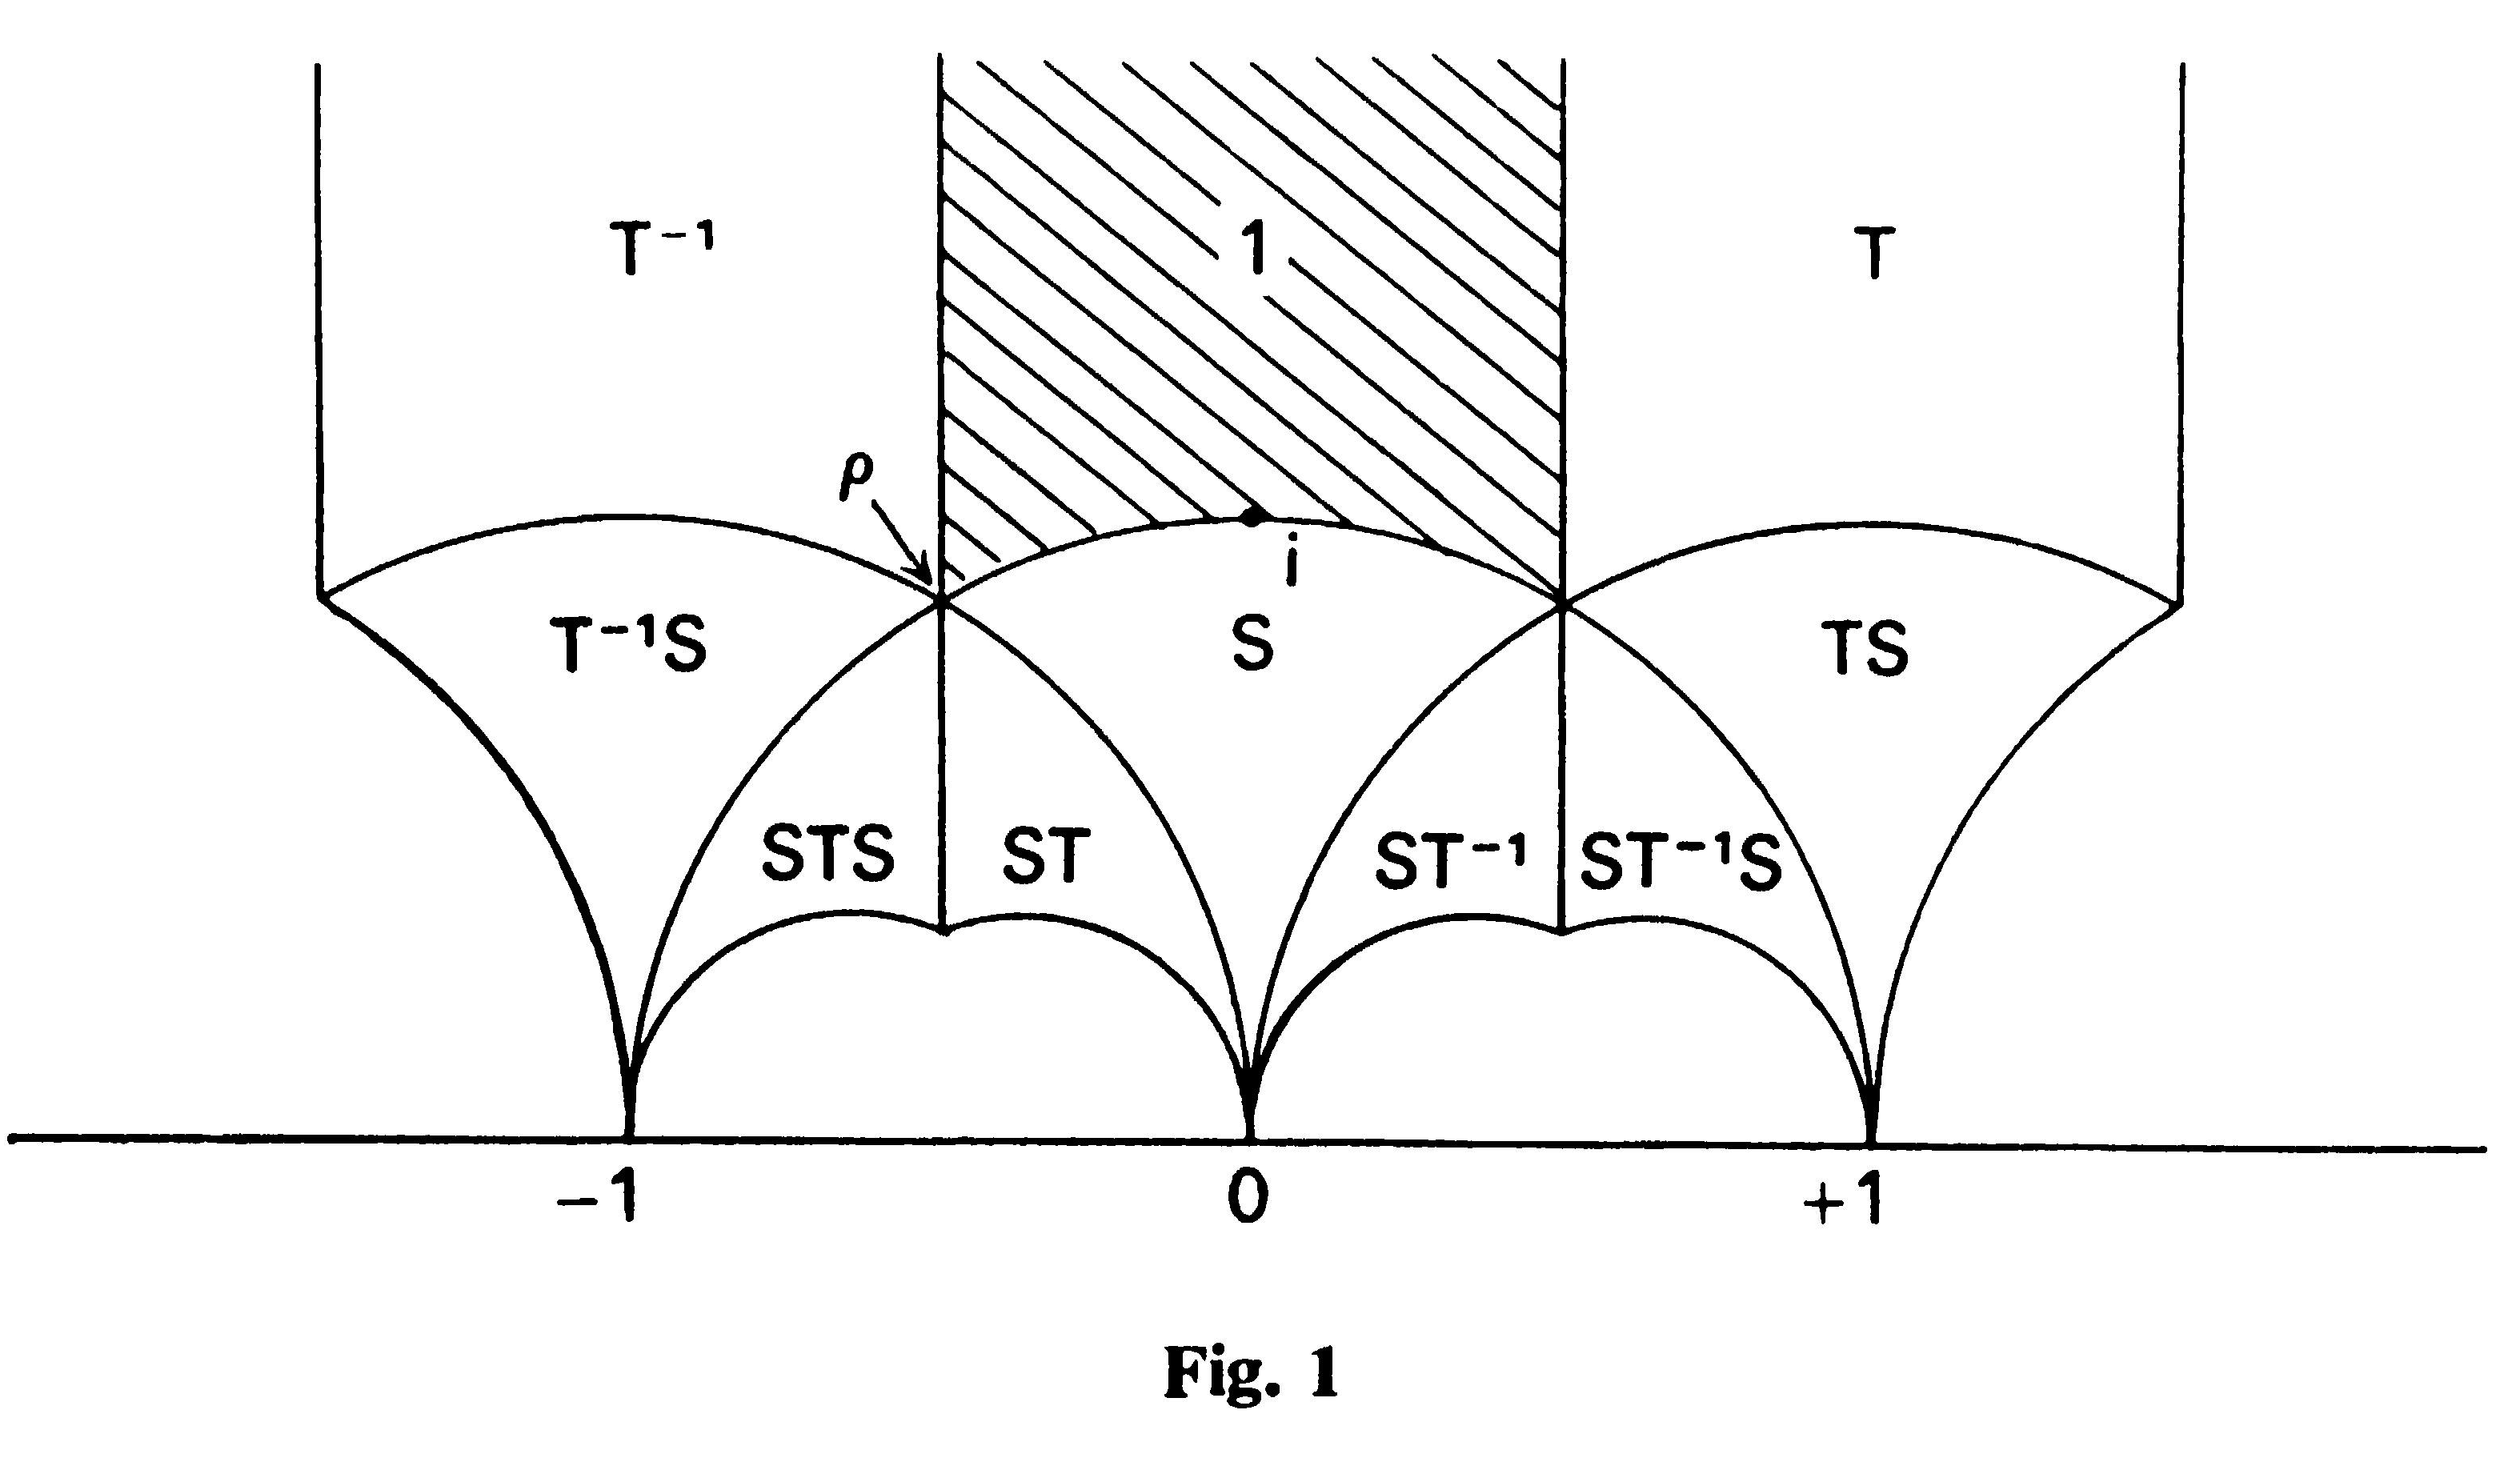
\includegraphics[width=10cm, height=6.5cm]{pics/fun-domain-SL2.png}
  \end{center}

\end{frame}

%% frame

\begin{frame}
\frametitle{$M(\SL_2(\BZ)) \cong \BC[E_4,E_6]$}
%\begin{center}
   % $K = -2 \infty + \frac{1}{2}P_1 + \frac{1}{3} P_2 + \infty$
  %\end{center}


\begin{center}
\begin{tabular}{ |c| c| c|}
\hline
$d$  & $\dim M_{2k}(\SL_2(\BBZ))$  \\ 
\hline
0& 1 \\ 
1& 0 \\  
2& 1  \\
3& 1  \\
4& 1  \\
5& 1  \\
6& 2   \\
\hline
\end{tabular}
\end{center}

\[
	M(\SL_2(\BZ)) \cong \BC[E_4,E_6]
\]
\end{frame}

%%frame

\begin{frame}

\begin{block}{Goal}
Let $\Gamma$ be a congruent subgroup of $\SL_2(\BBZ)$ (or any Fuchsian group with finite quotient). \\
Can we bound the degrees of generators and relations of $\overline{\Gamma \backslash \mathbb{H}}$?
\end{block}

\end{frame}

%% frame

\begin{frame}{Translation to Geometry (Kodaira--Spencer)}
\begin{block}{Modular Curves}
\begin{enumerate}
  \item $\sy = \Gamma \backslash \BH$
  \item $\sx = \sy \cup \Delta = \overline{\Gamma \backslash \BH}$
\end{enumerate}
\end{block}

\begin{block}{Kodaira--Spencer}
\begin{align*}
  M_k(\Gamma) &\cong H^0(\sx, \Omega^1(\Delta)^{\otimes \frac{k}{2}}) \\
	f(z) &\mapsto f(z)\, dz^{\otimes \frac{k}{2}}
\end{align*}
\end{block}

\begin{block}{Log Spin Canonical Ring}
%but this is something proved in VZB following from K--S
\begin{align*}
  M(\Gamma) &\cong R_{\sx,\Delta} := \bigoplus_{k \geq 0} H^0(\sx, \Omega^1(\Delta)^{\otimes \frac{k}{2}}) \\
\end{align*}
\end{block}

\end{frame}

%%%%%%%%%%%%%%%%%%%%   Stacky Curves Section   %%%%%%%%%%%%%%%%%%%
\section{Stacky Curves}

\begin{frame}{Stacky Curves}
\begin{defn}
A \textbf{stacky curve} $\sx$ over $\Bk$
is informally
	\begin{itemize}
		\item Informally: a curve where some points have ``fractional order''
		\item Formally: Deligne-Mumford Stack satisfying...
	\end{itemize}
\end{defn}

\begin{fact}
Let $X$ be the {\bf coarse space} of $\sx$.
\[
	K_{\sx} = K_X + \sum \frac{e_P-1}{e_P} P
\]
\end{fact}
\end{frame}

%% frame

\begin{frame}{Fractional Divisors}
%\begin{figure}
\begin{equation} \label{pic:M-curve} \notag
% \begin{center}
  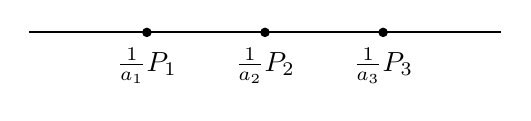
\begin{tikzpicture}
    \draw[thick] (-3,0) -- (3,0);
    % \draw plot[only marks,mark=*] coordinates{(0,0)};
    % \draw plot[only marks,mark=*] coordinates{(-1.5,0)};
		
    %\filldraw[draw=black,fill=black] (-1.5,0) node [below=2pt]{$\mu_{a_1}$} circle (1.5pt);
		%\filldraw[draw=black,fill=black] (0,0) node [below=2pt] {$\mu_{a_1}$} circle (1.5pt);
    %\filldraw[draw=black,fill=black] (1.5,0) node [below=2pt] {$\mu_{a_1}$} circle (1.5pt);
		
		\filldraw[draw=black,fill=black] (-1.5,0) node [below=2pt]{$\frac{1}{a_1}P_1$} circle (1.5pt);
		\filldraw[draw=black,fill=black] (0,0) node [below=2pt] {$\frac{1}{a_2}P_2$} circle (1.5pt);
		\filldraw[draw=black,fill=black] (1.5,0) node [below=2pt] {$\frac{1}{a_3}P_3$} circle (1.5pt);
		
    % \filldraw[draw=white,fill=white] (0,-1) node {$\mu_3$} circle
    % (8pt); don't do this
  \end{tikzpicture}
%\end{center}
\end{equation}

\begin{rem}
  \begin{itemize}
  \item Divisors are now \textbf{fractional}.
  \item $D = D_0 + \frac{n_{1}}{a_1}P_1 + \frac{n_{2}}{a_2}P_2 + \frac{n_{3}}{a_3}P_{3}$
  \end{itemize}
\end{rem}

%\begin{block}{General Description of ``Stacky'' Divisors}
%\[
%	\di \sx = \left(\bigoplus_{P\notin \{P_1, \ldots, P_r\}} \langle 
%	P \rangle \right) \oplus \left(\bigoplus_{i = 1}^r \left \langle 
%	\frac{1}{e_i}P_i \right \rangle \right) \subseteq \BQ \otimes \di X.
%\]
%\end{block}
\end{frame}

%% frame

\begin{frame}{Log Spin Canonical Divisors}
We can equip stacky curves with an effective divisor $\Delta$.

%\begin{defn}
%Divisor $\Delta$ is a \textbf{log divisor} if it is a sum of distinct
%points each with trivial stabilizer. Let $\delta := \deg \Delta$
%denote its degree.
%\end{defn}


%\begin{defn}
%If $\sx$ has coarse space $X$ of genus $g$, then we say $\sx$ has
%\textbf{signature} $\sigma = (g; e_1, \ldots, e_r; \delta)$.
%\end{defn}


\begin{defn}
Suppose $\halfcan \in \di
\sx$ satisfies $2 \halfcan \sim K_X + \Delta + \sum_{i = 1}^{r}
\frac{e_i - 1}{e_i} P_i$.  We call $\halfcan$ a
\textbf{log spin canonical divisor} on $(\sx, \Delta)$.
\end{defn}

\begin{block}{Fact}
\[
	\halfcan \sim \sum_{i = 1}^{r} \frac{e_i - 1}{2e_i} P_i
	+ \sum_{j = 1}^{\ell} Q_j
\]
\end{block}

\end{frame}

%% frame

\begin{frame}{Log Spin Canonical Rings}

%\begin{defn}
%If divisor $D \in \di \sx$ and $D = \sum_{i = 1}^{n} \alpha_i P_i$
%with $\alpha_i \in \BQ$, the floor of a divisor $\lfloor D
%\rfloor$ is defined to be $\lfloor D \rfloor := \sum_{i = 1}^{n}
%\lfloor \alpha_i \rfloor P_i$.
%\end{defn}

%\begin{defn}
%Let $\sx$ be a stacky curve with coarse space $X$.
%If $D \in \di \sx$ is a divisor, then we define

%\[
%	H^0(\sx, D) := H^0(X, \lfloor D \rfloor).
%\]
%\end{defn}

\begin{defn}
The {\bf log spin canonical ring} of $(\sx, \Delta, \halfcan)$ is
\[
	R(\sx, \Delta, \halfcan) := \bigoplus_{k \geq 0} H^0(X, \lfloor k \halfcan \rfloor).
\]
\end{defn}

\begin{itemize}
\item Not ad hoc
\end{itemize}

\end{frame}

%%%%%%%%%%%%%%%%%%%%   Main Result Section   %%%%%%%%%%%%%%%%%%%
\section{Main Result}

\begin{frame}{Main Problem}
%\begin{block}{Setup}
%Let $\sx$ be a stacky curve of genus 0 with stacky points $P_1, \ldots P_r$
%Recall $2 \halfcan \sim K_X + \Delta + \sum_{i = 1}^{r}
%\frac{e_i - 1}{e_i} P_i$.
%\end{block}

\begin{block}{Goal}
%Let $(\sx, \Delta, \halfcan)$ be a log spin curve.
Bound the degrees of generators and relations of log spin
canonical rings

\[
	R(\sx, \Delta, \halfcan) = \bigoplus_{k \geq 0} H^0(X, \lfloor k \halfcan \rfloor).
\]
\end{block}
\end{frame}

\begin{frame}{Example of Log Spin Canonical Ring}
Let $(\sx, \Delta, \halfcan)$ be genus 0 such that $\halfcan \sim -\infty + \frac{1}{3} P_1 +
\frac{3}{7} P_2 + \frac{3}{7} P_3$. 
%where $P_1, P_2,$ and $P_3$ are distinct points.

\vspace*{-0.5cm}
\begin{align*}
	&R(\sx, \Delta, \halfcan) = \Bk[x_{7, 2}, x_{7, 1}, x_{5, 1}, x_{3, 1}] / \langle f, g \rangle \\
	&f = a_1 x_{5, 1}^2 + a_2 x_{7, 2} x_{3, 1} + a_3 x_{7, 1} x_{3, 1} 
	&\text{ in degree $10$} \\
	&g = b_1 x_{7, 2}^2 + b_2 x_{7, 2} x_{7, 1} + b_3 x_{7, 1}^2
	+ b_4 x_{5, 1} x_{3, 1}^3  &\text{ in degree $14$}
\end{align*}

\begin{figure}
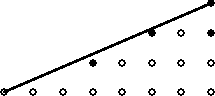
\includegraphics{pics/spin-377-pic-pics.pdf} \\
\caption{Generators in the $(\deg z, -ord_{P_2}(z))$ lattice}
\end{figure}

\end{frame}

%% frame

\begin{frame}{Previous Work}
\begin{block}{Bounds (O'Dorney)}
Weakly bounds generator and relations degrees in terms of
the least common multiples of the $e_i$'s when $g = 0$.
\end{block}

\begin{block}{Theorem (Voight and Zureick-Brown)}
Bounds generator degrees by $6
\cdot \max(3, e_1, \ldots, e_r)$ and relation degrees by $12 \cdot \max
(3, e_1, \ldots, e_ r)$ when $\halfcan$ is effective.
\end{block}

\begin{block}{Application to Previous Example}
\begin{itemize}
\item O'Dorney: generators in degrees $\leq 238$, relations in degrees $\leq 385$
\item Voight--Zureick-Brown: generators in degrees $\leq 42$, relations in $\leq 84$.
\end{itemize}
\end{block}

\end{frame}

%%frame

\begin{frame}{Main Result}
\begin{thm}
\label{thm:main}
Log spin curve $(\sx, \Delta, \halfcan)$ with stacky points $P_1, \ldots P_r$. \\
Let $e := \max(5, e_1, \ldots, e_r)$.

The log spin canonical ring 
\[
	R(\sx, \Delta, \halfcan) = \bigoplus_{k \geq 0} H^0(X, \lfloor k \halfcan \rfloor)
\]

\noindent
is generated in degrees at most $e$ with relations generated in
degrees up to $2e$ with a finite list of exceptions.
\end{thm}
\end{frame}

%% frame

\begin{frame}{Main Idea of Proof}
%\begin{block}{Setup}
%Let $(\sx', \Delta, \halfcan')$ be a log spin curve over a perfect
%field $k$, so that $\sx$ has signature $\sigma := (g; e_1, \ldots,
%e_r; \delta)$. Recall $\halfcan \sim \sum_{i = 1}^{r} \frac{e_i - 1}{2e_i} P_i
%+ \sum_{j = 1}^{\ell} Q_\ell$.
%\end{block}

\begin{block}{Inductive Step}
Given generators and relations of $(\sx', \Delta, \halfcan')$, we can deduce generators and relations in $(\sx, \Delta, \halfcan)$, in the following situations:
\begin{itemize}
\item $(\sx, \Delta, \halfcan)$ looks like $(\sx', \Delta, \halfcan')$, except with one added stacky point
\item $(\sx, \Delta, \halfcan)$ looks like $(\sx', \Delta, \halfcan')$, except with one stabilizer order $e_i$ incremented by 2
\end{itemize}
\end{block}

\begin{rem}
These inductive methods are explicit!
\end{rem}

%\begin{itemize}
%\item Induction on adding points \\
%\item Induction on raising stabilizer order \\
%\item Base cases
%\end{itemize}
\end{frame}

\begin{frame}{Applications}
%Let $\Gamma$ be a Fuchsian group and $\sx$ the stacky curve
%associated to $\Gamma \backslash \BH$ with signature $\sigma
%:= (g; e_1, \ldots, e_r; \delta)$. Let $e_\ell := \max(\ell, e_1, \ldots, e_r)$.
%
%The ring of modular forms $M(\Gamma)$ is generated as a $\BC$-algebra
%
%\begin{block}{Main Corollary}
%\begin{itemize}
%\item if $M_k(\Gamma) = 0$ for all odd $k$:
%by elements of
%degree at most $6 e_3$ with relations
%generated in degrees at most $12 e_3$ \\
%\end{itemize}

%\begin{itemize}
%\item otherwise: by elements of degree at most $e_5$ with
%relations generated in degrees at most $2 e_5$ with a
%finite list of exceptional signatures $\sigma$.
%\end{itemize}
%\end{block}

\begin{block}{Corollary}
Suppose $\Gamma \subseteq \SL_2(\BZ)$ is a congruence subgroup
\begin{itemize}
\item General: $M(\Gamma)$ is generated up to degree $6$, relations up to degree $12$. 
\item Some nonzero odd weight modular form: $M(\Gamma)$ is generated up to degree $5$, relations up to degree $10$.
\end{itemize}
\end{block}

\begin{block}{Remark}
We have generalized this result to general Fuchsian groups.
\end{block}
\end{frame}

%%%%%%%%%%%%%%%%%%%%   Further Research Section   %%%%%%%%%%%%%%%%%%%
%\section{Further Research} 
%
%\begin{frame}{Further Research}
%\begin{itemize}
%\item General structure theorem for a presentation of $R_{L_X}$ when genus $\ge 2$. \\
%\item Fractional weight divisors $D$ satisfying $nD \sim K$. \\
%\item Rework proof to find generic initial ideal \\
%\end{itemize}
%Peter: I only included the first 3 of the five further questions, to save space.
%
%\end{frame}

%%%%%%%%%%%%%%%%%%%%   Acknowledgments Section   %%%%%%%%%%%%%%%%%%%

%frame probably unnecessary
\begin{frame}
\frametitle{Acknowledgments}
\begin{itemize}
	\item David Zureick-Brown
	\item Ken Ono
	\item Others
	\begin{itemize}
		\item Brian Conrad
		\item Jorge Neves
		\item John Voight
		\item Shou-Wu Zhang
		%\item Ravi Vakil
		%\item Nadim Rustom
	\end{itemize}
\end{itemize}
\end{frame}

\end{document}





